% Template for ICASSP-2016 paper; to be used with:
%          spconf.sty  - ICASSP/ICIP LaTeX style file, and
%          IEEEbib.bst - IEEE bibliography style file.
% --------------------------------------------------------------------------
\documentclass[12pt]{article}
\usepackage{spconf, amsmath, graphicx, float}
\usepackage{scrlayer-scrpage}
\clearpairofpagestyles
\cfoot*{\pagemark}
% Example definitions.
% --------------------
\def\x{{\mathbf x}}
\def\L{{\cal L}}

% Title.
% ------
\title{Walmart Store Forecasting}
%
% Single address.
% ---------------
\name{Atom Group: Jifu Zhao (jzhao59), Jinsheng Wang (jwang278)}
\address{Nuclear, Plasma, and Radiological Engineering \\
              University of Illinois at Urbana-Champaign\\
		       Urbana, Illinois 61801, USA}

\begin{document}
%\ninept
%
\maketitle

\section{Introduction}
\quad\ In this project, our goal is to predict the weekly sales for each department in each store for Walmart. The original training data includes the historical data from 2010 - 02 to 2011 - 02.  The test data is from 2011 - 03 to 2012 - 10, totally 20 months. In each iteration, we will be given the historical training data and the previous month's data, then we are asked to predict the sales for the next month.

The data set contains multiple features, including Store, Dept, Date, Weekly\_Sales, IsHolday. After some initial analysis, we find that there are 81 unique departments and 45 unique stores. In this project, we first explore the given training data set. After some pre-processing methods, we applied three different models to predict the next month's sales. More details will be described in the following sections.

\section{Pre-processing}
After exploring the training dataset, 

In our R code, we loaded three libraries to simplify our task, including lubridate, forecast, plyr.


\section{Methods}

\subsection{Average from Nearby Weeks}
In our first model, Model 1, we basically choose the nearby three weeks to make prediction. For example, for a given store and department in week w, we find the corresponding data for the same department and store from the last year, then we choose the median of the sales from w - 1, w, w + 1 as the prediction.

\subsection{Time Series Forecasting}
In Method 2, we choose ts() to create a time series whose frequency is 52 and auto.arima() to forecast for a give step. More specially, for a given store and department, we first extract the data from previous years that is from the same department and store. Then we use the ts() function to create a time series whose frequency is 52. Finally, through feeding the time series into auto.arima(), we make the prediction that corresponding to next month's sales.

\subsection{Weighted Average of Model 1 and Model 2}
In this model, considering the long running time, we choose the weighted average of Model 1 and Model 2 as our third model, Model 3. Through some careful study, we find the the weight should be 0.7 for Model 1 and 0.3 for Model 2. The final expression for Model 3 is shown below:
\begin{equation}
Model \  3 = 0.7 \times Model \  1 + 0.3 \times Model \  2
\end{equation}


\section{Code Description}
\quad\ All of our code is contained in the file named mymain.R. 


There are basically three parts in the R file. At the very beginning, the code will automatically check whether or not the required packages/libraries are already installed. In the second part of the code, we do data preprocessing: first read the training and test data sets, then drop the useless variables and process the features to form the new feature space. For the last part, we mainly build our three model: Linear Regression, Lasso Regression and Random Forest model. These built models will make predictions and the results are saved into local file system as required by the project description.

Due to the amount of data to be looped, the code need a lot of time to run. As tested, the total running time is around 2 hours.

\section{Results}

To evaluate our model, we choose the metric described on Kaggle:
\begin{equation}
WMAE = \frac{1}{\sum_{i=1}^n w_i} \sum_{i=1}^n w_i | y_i - \hat{y}_i |
\end{equation}
where $n$ is the number of test cases, $\hat{y}_i$ is the predicted sales, $y_i$ is the actual sales and $w_i$ is the weights. For this project, we set $w=5$ if the week is a holiday and 1 otherwise. The final WMAE for three models are shown in Table~\ref{result}.

\begin{table}[htb]
 \caption{Summary of Models} \label{result}
 \vspace{0.1in}
\begin{center}
  \begin{tabular}{  c  c  }
  
    \hline
    Model          &WMAE     \\ \hline
    Model 1         & 2093.603    \\ \hline
    Model 2         & 2395.633    \\ \hline
    Model 3         & 1956.629    \\ \hline
  \end{tabular}
\end{center}
\end{table}

From Table~\ref{result}, one can find that, Model 1 and Model 2 performs similar to each other. Through weighted averaging, the final model, Model 3, performs better than Model 1 and Model 2.

\subsection*{Acknowledgement}

%\begin{figure}[htb]
%\centering
%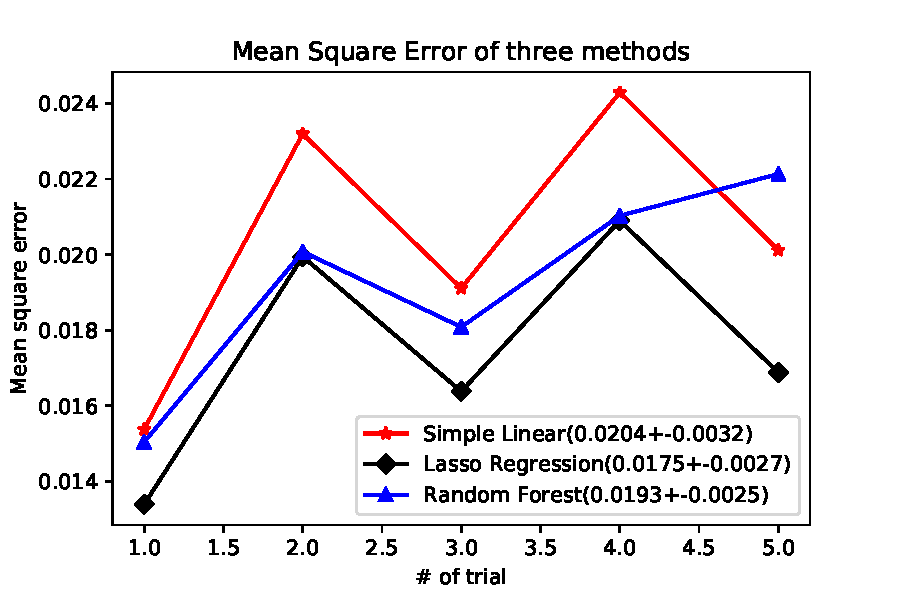
\includegraphics[width=0.45\textwidth]{./figures/MSE_3_methods.pdf}
%\caption{Results of different models}
%\label{fig:autoencoder}
%\end{figure}

\quad\ The authors would like to thank Xichen Huang for his tutorial notebook on Piazza and David Thaler for his online code.

\vfill\pagebreak

% References should be produced using the bibtex program from suitable
% BiBTeX files (here: strings, refs, manuals). The IEEEbib.bst bibliography
% style file from IEEE produces unsorted bibliography list.
% -------------------------------------------------------------------------
%\bibliographystyle{IEEEbib}%\bibliography{strings,refs}
%\bibliography{strings}

\end{document}